% ==============================================================================
% ================================== AUFGABE 5 ================================
% ==============================================================================

\chapter{Aufgabe 5: Retrospektive Analyse des Gesprächsverlaufs} 
\label{sec:aufgabe5}

\section{Systematische Rekonstruktion der Gesprächsdynamik}
Um das Fehlschlagen der Interaktion wissenschaftlich zu erklären, ist der reale Gesprächsverlauf rückblickend in seinen Phasen, Umschlagpunkten und ursächlichen Triebkräften zu analysieren. Die Eskalation vollzog sich nicht zufällig, sondern folgte einer klaren sozialpsychologischen Gesetzmäßigkeit, bei der sachorientierte Problemlösungsversuche zunehmend von emotionalen Abwehr- und Machtmechanismen verdrängt wurden \cite[S.~24]{5}.

\section{Identifikation des kritischen Wendepunkts (Tipping Point)}
Der Wendepunkt, an dem die Kommunikation von einer (wenn auch angespannten) Sachdiskussion in eine unkontrollierbare Beziehungs- und Machteskalation umschlägt, lässt sich im Dialogskript präzise lokalisieren:

\begin{quote}
\textit{Dienstleister (D):} „[...] Um das Projekt dennoch voranzutreiben, habe ich Ihnen in einer E-Mail [...] transparent mitgeteilt, dass wir, wenn keine Rückmeldung erfolgt, vorübergehend eigene Annahmeparameter einsetzen müssen.“ \\
\textit{Kundin (K):} „Hören Sie auf, mir etwas von E-Mails zu erzählen. Sie wollen sich doch nur rausreden. [...] Jetzt läuft es nicht, und Sie schieben es auf mich. Das ist erbärmlich. Sie sind einfach nicht kompetent genug für diese Aufgabe.“
\end{quote}

\textbf{Analyse der Wendestelle:}
Bis zu diesem Zeitpunkt bestand auf Seiten der Kundin zwar eine erhebliche emotionale Aufladung, die Interaktion verblieb jedoch vordergründig auf der Fragestellung der Fehlerursache. Mit dem detaillierten Verweis des Dienstleisters auf die gesendeten E-Mails und die Versäumnisse bei den Datenlieferungen der Kundin wechselt der Fokus schlagartig:
\begin{itemize}
    \item Die Kundin interpretiert die faktische Aufzählung der Datumsangaben nicht als sachliche Aufklärung, sondern als einen \textbf{direkten Angriff auf ihre berufliche Kompetenz} und ihre Integrität vor dem Hintergrund des herrschenden Vorstandsdrucks.
    \item Anstatt den Ball aufzunehmen und die Versäumnisse einzuräumen, geht die Kundin zur Verhaltensweise des \textbf{Gegenangriffs und der persönlichen Entwertung} über („Sie sind einfach nicht kompetent genug für diese Aufgabe“). An dieser Stelle bricht der Inhaltsaspekt vollends zusammen.
\end{itemize}

\section{Tiefere Ursachen des Konfliktausbruchs}
Das Umschlagen der Situation ist das Ergebnis mehrschichtiger Ursachenfaktoren, die bereits vor dem physischen Zusammentreffen im Verborgenen wirkten:

\subsection{Struktureller Leistungs- und Termindruck auf Kundenseite}
Ein primärer Konflikttreiber liegt in der exogenen Bedrohungslage der Kundin. Als Prozessverantwortliche steht sie unter massiver Beobachtung durch den Vorstand. Die Fehlfunktionen im Automatisierungsmodul gefährden die Abnahme der finanziellen Nachprüfung. Aus der Angst vor eigenen Sanktionen entsteht ein hoher innerer Druck, der sich im Gespräch als aggressive Projektion auf den Dienstleister entlädt \cite[S.~8--9]{5}.

\subsection{Unklare Rollenerwartungen und Beziehungsstörung}
Zwischen den Beteiligten bestand ein unaufgelöster Rollenkonflikt \cite[S.~7]{5}. Während die Kundin das Modell einer starren, komplementären Hierarchie einforderte (Dienstleister als reiner Erfüllungsgehilfe, der Lücken geräuschlos zu schließen hat), agierte der Entwickler aus dem Selbstverständnis eines gleichberechtigten Experten, der eine partnerschaftliche Mitwirkung und fristgerechte Zuarbeit einfordert \cite[S.~18]{5}.

\subsection{Asymmetrischer Informationsstand und Fehlannahmen}
Durch das eigenmächtige Schätzen der 47 Standardparameter zur Einhaltung des Abnahmetermins schuf der Dienstleister eine Scheinqualität. Der Kundin war nicht bewusst, dass das Modul auf Schätzwerten basierte. Die plötzliche Konfrontation mit Abweichungen erzeugte bei ihr das Gefühl des getäuschten Vertrauens.

\section{Analyse der Eskalationsmechanismen}

\subsection{Einordnung in die Eskalationsstufen nach Glasl}
Die Entwicklung der Interaktion lässt sich mithilfe des neunstufigen Phasenschemas nach Glasl systematisch nachzeichnen (Glasl, zit. n. \cite[S.~33--40]{5}):

\begin{figure}[H]
\centering
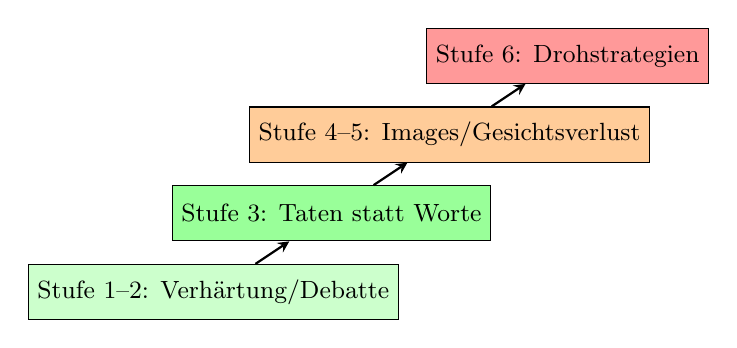
\begin{tikzpicture}[
    escstep/.style={rectangle, draw, minimum width=3.5cm, minimum height=0.7cm,
                    align=center, font=\small},
    escarrow/.style={->, thick, >=stealth}
]
    \node[escstep, fill=green!20]  (s1) at (0,0)   {Stufe 1–2: Verhärtung/Debatte};
    \node[escstep, fill=green!40]  (s2) at (1.5,1) {Stufe 3: Taten statt Worte};
    \node[escstep, fill=orange!40] (s3) at (3,2)   {Stufe 4–5: Images/Gesichtsverlust};
    \node[escstep, fill=red!40]    (s4) at (4.5,3) {Stufe 6: Drohstrategien};
    \draw[escarrow] (s1) -- (s2);
    \draw[escarrow] (s2) -- (s3);
    \draw[escarrow] (s3) -- (s4);
\end{tikzpicture}
\caption{Eskalationsstufen nach Glasl und ihre Entsprechung im Dialogskript}
\label{fig:glasl-eskalation}
\end{figure}

\begin{itemize}
    \item \textbf{Stufe 1 bis 2 (Verhärtung und Debatte):} Zu Gesprächsbeginn treffen gegensätzliche Standpunkte aufeinander (Kritik am Modul vs. Hinweis auf fehlende Zuarbeit).
    \item \textbf{Stufe 3 (Taten statt Worte):} Durch das Aufstehen, Tischschlagen und Vorhalten der E-Mail-Historie schlägt die verbal-argumentative Ebene in demonstratives Druckverhalten um (Glasl, zit. n. \cite[S.~36--37]{5}).
    \item \textbf{Stufe 4 bis 5 (Images/Koalitionen und Gesichtsverlust):} Mit der persönlichen Beschimpfung („dahergelaufener angeblicher Programmierer“) verlässt die Kundin die Sachebene vollständig. Es geht fortan um die Entwertung des Gegenübers und die Zerstörung des fachlichen Ansehens (Glasl, zit. n. \cite[S.~37--38]{5}).
    \item \textbf{Stufe 6 (Drohstrategien und Beziehungsabbruch):} Das Ultimatum („bis heute Abend“) und der finale Raumverlass mit Türknallen markieren den Übergang zur Stufe 6 (Drohung mit endgültigem Beziehungs- und Projektabbruch) (Glasl, zit. n. \cite[S.~39--40]{5}).
\end{itemize}

\subsection{Fehlsteuerung im Vier-Seiten-Modell nach Schulz von Thun}
Kiefer erklärt die Ursache für das Hochschaukeln zudem über das Vier-Seiten-Modell der Nachricht (Schulz von Thun, zit. n. \cite[S.~19--24]{3}):
\begin{itemize}
    \item \textbf{Aussage des Dienstleisters:} „Ich habe Ihnen am 8., 15. und 22. des letzten Monats konkrete Rückfragen per E-Mail geschickt.“
    \item \textbf{Sachebene:} Sachinformation über versendete Nachrichten und Daten.
    \item \textbf{Empfang auf Kundenseite (Beziehungs- und Appell-Ohr):} Die Kundin hört auf dem Beziehungsohr: „Du hast deinen Job nicht gemacht und bist schuld am Scheitern.“ Auf dem Appell-Ohr hört sie: „Gib endlich deine Fehler zu.“
\end{itemize}
Da die Kundin die Nachricht überwiegend mit dem emotional überempfindlichen Beziehungsohr dekodierte, reagierte sie nicht auf die Sachinformation, sondern mit einem Abwehrschlag gegen die gefühlte Entwertung (Schulz von Thun, zit. n. \cite[S.~21--22]{3}).

\subsection{Die drei Antriebsmechanismen der Eskalation}
Kiefer erklärt die Dynamik des Hochschaukelns präzise mit den drei Antriebsmechanismen nach Glasl (Glasl, zit. n. \cite[S.~30--33]{5}):
\begin{itemize}
    \item \textbf{Wachsende Streitpunktlawine:} Während der Dienstleister immer mehr sachliche Details (Daten, E-Mails, Lastenheft) aufführt, bringt die Kundin immer neue Vorwürfe ein (mangelnde Kompetenz, fehlendes Projektmanagement, „IT-Welt“). Beide Seiten reden zunehmend aneinander vorbei.
    \item \textbf{Arena-Ausweitung und Personifizierung:} Die Kundin zieht den Vorstand als Drohkulisse heran („Mein Vorstand hat heute Morgen den Projektstatus angefordert“). Der Konflikt wird von der Sachebene auf die Beziehungsebene und die organisationale Ebene verschoben. Gleichzeitig personifiziert sie den Konflikt auf den Dienstleister („Du elendes Element“).
    \item \textbf{Pessimistische Antizipation und selbsterfüllende Vorhersage:} Die Kundin erwartet das Schlimmste (drohende Sanktionen durch den Vorstand) und reagiert entsprechend aggressiv. Durch ihr aggressives Verhalten provoziert sie genau die Reaktion des Dienstleisters (Rechtfertigung, Rückzug), die sie als Bestätigung ihrer negativen Erwartung interpretiert.
\end{itemize}

\subsection{Selbstansteckung als übergreifender Mechanismus}
Kiefer beschreibt, dass die Eskalation dem Mechanismus der Selbstansteckung nach Glasl folgt (Glasl, zit. n. \cite[S.~42--43]{5}). Aus der anfänglichen Sachdifferenz (fehlerhaftes Modul vs. fehlende Daten) entwickelt sich eine Beziehungsstörung (gegenseitige Entwertung). Diese wiederum polarisiert die Sachstandpunkte (K fordert „machen Sie, dass es funktioniert“, D pocht auf das Lastenheft), bis schließlich der Konflikt über den Konflikt („Wer ist schuld?“) den Konflikt über die Konfliktlösung („Wie gehen wir vor?“) vollständig verdrängt.

\section{Fazit der Analyse}
Das Gespräch ist gescheitert, weil der Dienstleister versuchte, eine auf der Beziehungsebene hochexplosive Situation mit rein digitalen Sachargumenten (E-Mail-Protokolle, Daten) zu lösen. Dadurch fühlte sich die ohnehin unter Vorstandsspannung stehende Kundin in die Enge getrieben. Der resultierende Gesichtsverlust veranlasste sie zum Ausbruch aus der Kommunikation mittels verbaler Aggression und anschließendem Raumverlass. Die Eskalation folgte dabei exakt den von Glasl beschriebenen Mechanismen der Streitpunktlawine, der Arena-Ausweitung und der pessimistischen Antizipation sowie dem übergreifenden Prinzip der Selbstansteckung (Glasl, zit. n. \cite[S.~30--33]{5}).

% ==============================================================================
% ================================== AUFGABE 5 ================================
% ==============================================================================